\chapter{Huấn luyện, thử nghiệm và đánh giá}

Chương này sẽ trình chi tiết các kịch bản thử nghiệm để đánh giá hiệu quả của giải pháp co dãn đa cấp độ chủ động được đề xuất trong chương 3, hệ thống triển khai, đánh giá và theo dõi được nêu rõ tại chương 4. Kết quả thử nghiệm sẽ được đánh giá, phân tích và so sánh nhằm đưa ra kết luận về hiệu năng và hiệu suất của giải pháp hệ thống được để xuất.

\section{Yêu cầu của hệ thống}

Đầu tiên, ta đưa ra các tiêu chí yêu cầu của hệ thống làm cơ sở để triển khai các kịch bản thử nghiệm và đánh giá, phân tích sau này.

\begin{itemize}
    \item Cân bằng giữa việc mở rộng và thu hẹp: Đảm bảo không mở rộng quá mức khi hệ thống có chịu được tải, do môi trường triển khai trên hệ thống điện đoán đám mây, bất kỳ tài nguyên không hợp lý nào đều sẽ gây ra lãng phí. Không thu hẹp quá nhiều khiến hệ thống thiếu tài nguyên xử lý, gây ảnh hưởng nghiêm trọng đến trải nghiệm người dùng.
    \item Hiệu năng ổn định: Hệ thống hoạt động ổn định, xuyên suốt.
    \item Tự động cấu hình lại tài nguyên: Hệ thống cần có khả năng tự động cấu hình lại các tài nguyên như máy chủ ảo hoặc container mà không cần sự can thiệp thủ công.
    \item Giám sát hiệu suất: Hệ thống phải có khả năng theo dõi liên tục các chỉ số như CPU, bộ nhớ, băng thông mạng và độ trễ.
    \item Hệ thống có khả năng co/dãn các supervisor.
\end{itemize}

\paragraph{Cấu hình của các supervisor xử lý dữ liệu}

\begin{itemize}
    \item Mỗi supervisor có 600 Mb RAM và 1 core CPU tương ứng với 1 worker port: 6700.
    \item Số lượng supervisor tối đa là 5 và tối thiểu là 2.
\end{itemize}

\paragraph{Đánh giá sơ bộ}

Nhằm đơn giản hóa việc đánh giá, đồ thị tỷ lệ sử dụng bộ nhớ được bổ sung thêm 3 đường tham chiếu, tương ứng từ lớn đến nhỏ là 90\%, 60\% và 20\%. Tại mức tỷ lệ sử dụng bộ nhớ

\begin{itemize}
    \item 90\%: Supervisor đang sử dụng quá nhiều bộ nhớ, khả năng cao trong tương lai sẽ tiếp tục tăng và gây quá tải bộ nhớ làm tăng độ trễ của hệ thống.
    \item 60\%: Supervisor đang sử dụng bộ nhớ ở mức lý tưởng.
    \item 20\%: Supervisor đang gây lãng phí tài nguyên do mức tỷ lệ sử dụng bộ nhớ này tương đương với tiến trình hệ thống supervisor sử dụng, có nghĩa đóng góp của supervisor là không có hoặc không đáng kể.
\end{itemize}

Tại đồ thị số lượng tin gửi đi của spout, đường đồ thị thường có dạng tăng tuyến tính từ 0 đến một ngưỡng nào đó, lý do là bởi Storm UI thu thập dữ liệu theo cửa sổ thời gian mà cụ thể ở đây là 10 phút, vì vậy các đường tăng tuyến tính có thể được hiểu rằng spout đang truyền tin với tốc độ không đổi.

\section{Các kịch bản thử nghiệm}

\paragraph{Kịch bản thử nghiệm 1}

Đây là kịch bản chung dùng cho cả hai giai đoạn huấn luyện và thử nghiệm. Dữ liệu được gửi đến MQTT sẽ có các cấu hình như sau.

\begin{itemize}
    \item Gửi dữ liệu các tòa nhà 1, 2.
    \item Gửi thêm dữ liệu các tòa nhà 3, 6.
    \item Gửi thêm dữ liệu các tòa nhà 4, 5.
    \item Dừng gửi dữ liệu các tòa nhà 1, 6.
    \item Dừng gửi dữ liệu các tòa nhà 2, 4.
    \item Gửi thêm dữ liệu tòa nhà 6.
    \item Dừng gửi dữ liệu toàn bộ các tòa nhà.
\end{itemize}

\begin{figure}[H]
    \centering
    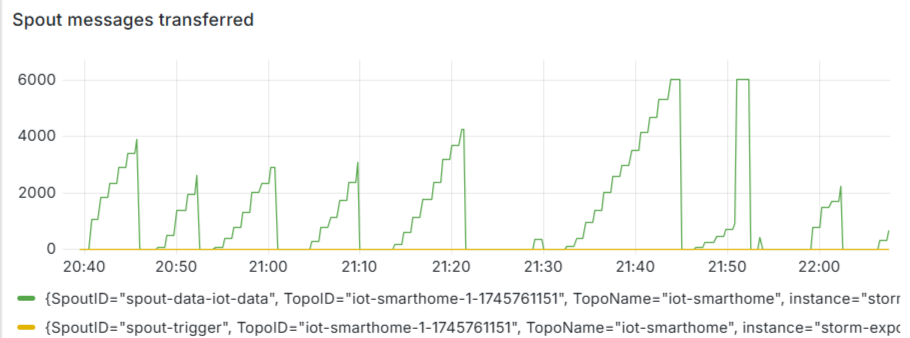
\includegraphics[width=\textwidth]{evaluation-01-messages-transferred.png}
    \caption{Theo dõi số lượng gói tin được gửi từ các spout trong giai đoạn huấn luyện}
\end{figure}

\begin{figure}[H]
    \centering
    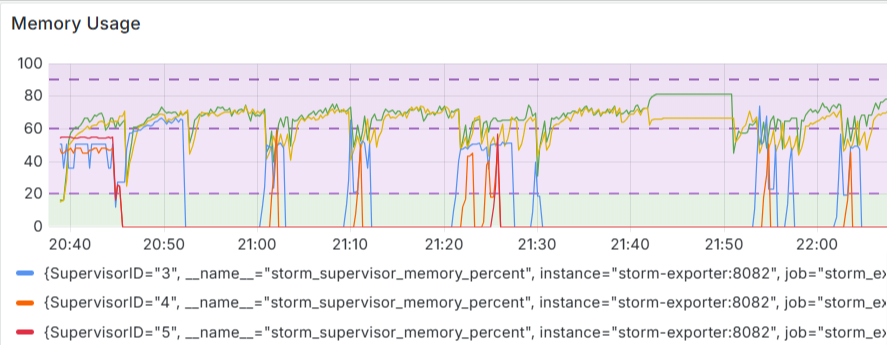
\includegraphics[width=\textwidth]{evaluation-01-memory-percent.png}
    \caption{Theo dõi tỷ lệ xử dụng bộ nhớ của các supervisor trong giai đoạn đánh giá}
\end{figure}

Có thể thấy hệ thống có thể tối ưu tỷ lệ sử dụng bộ nhớ khá tốt khi các supervisor đều có tỷ lệ sử dụng bộ nhớ quanh khoảng lý tưởng là 60\%.

\begin{figure}[H]
    \centering
    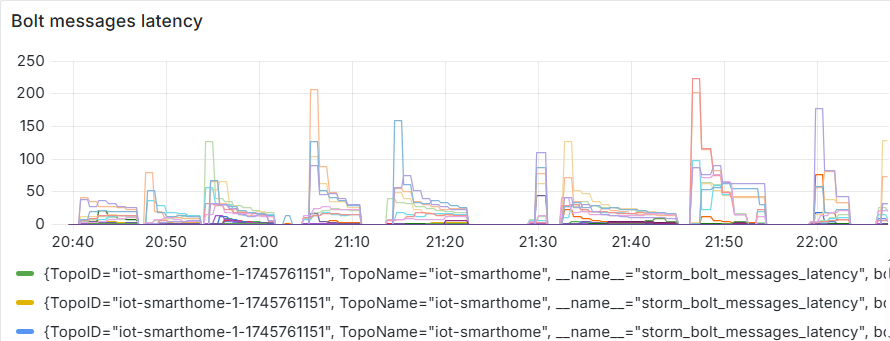
\includegraphics[width=\textwidth]{evaluation-01-bolt-messages-latency.png}
    \caption{Theo dõi độ trễ của các gói tin từ các bolt}
\end{figure}

\begin{figure}[H]
    \centering
    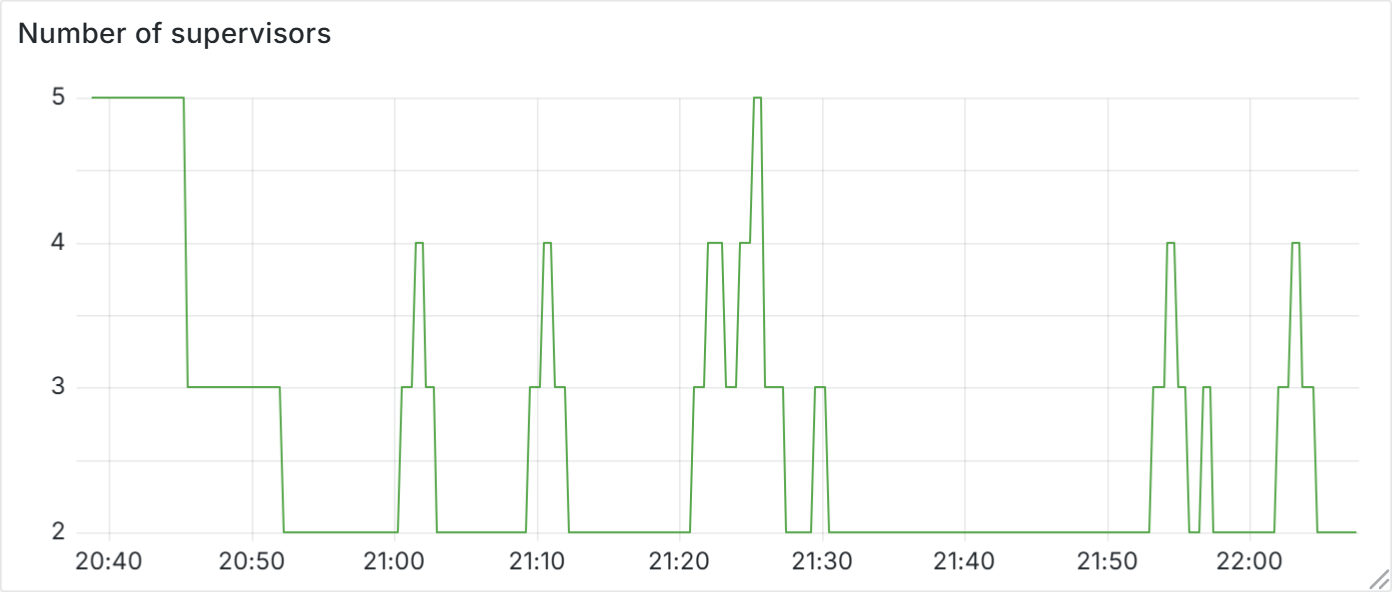
\includegraphics[width=\textwidth]{evaluation-01-number-of-supervisors.png}
    \caption{Theo dõi số lượng supervisor}
\end{figure}

Có thể nhận thấy, hệ thống đã có thể co/dãn số lượng supervisor để đáp ứng nhu cầu tải của hệ thống, khi độ trễ của gói tin của các bolt tăng cao, hệ thống đã đáp ứng bằng cách tăng số lượng supervisor lên để giảm tải khối lượng công việc cần xử lý của từng supervisor. Ví dụ, tại các thời điểm 20:56 và 21:06, độ trễ của các bolt tăng cao đột biến thì tại các thời điểm 21:00 và 21:09 hệ thống đã tăng liên tục từ 2 supervisor lên 4 supervisor để giảm tải giữa các supervisor. Tuy nhiên, có thể nhận thấy tốc độ phản hồi vẫn chưa đủ nhanh, đó là do
Tuy nhiên, lượng dữ liệu vẫn chưa phải đủ lớn để ta có thể nhìn thấy rõ được tác động của hệ thống đến với việc quản lý tài nguyên của ứng dụng SmartHome.